\section{Generowanie raportu}

Następnym ekran umożliwia wygenerowania raportu w formacie arkusza kalkulacyjnego na podstawie uzupełnionej bazy danych. W związku z tym w Power Apps przygotowano mechanizm łączący dane z trzech list SharePoint, które następnie są przesyłane do Power Automate, gdzie podlegają dalszemu przetwarzaniu. Wynikiem tego jest kompletny arkusz Excel, który jest zapisywany na platformie SharePoint.

\subsection{Łączenie danych z list}

W celu określenia, roku i indykacji których ma dotyczyć raport, wprowadzono kontrolki \emph{Dropdown} po lewej stronie ekranu. Ich uzupełnienie skutkuje wygenerowaniem podglądu danych, który pozwala na walidację ich poprawności. Listing \ref{lst:combineddata} przedstawia kod odpowiedzialny za utworzenie kolekcji \emph{CombinedData}, która zawiera odpowiednio odfiltrowane informacje.

% \begin{figure}[H]
%     \centering
%     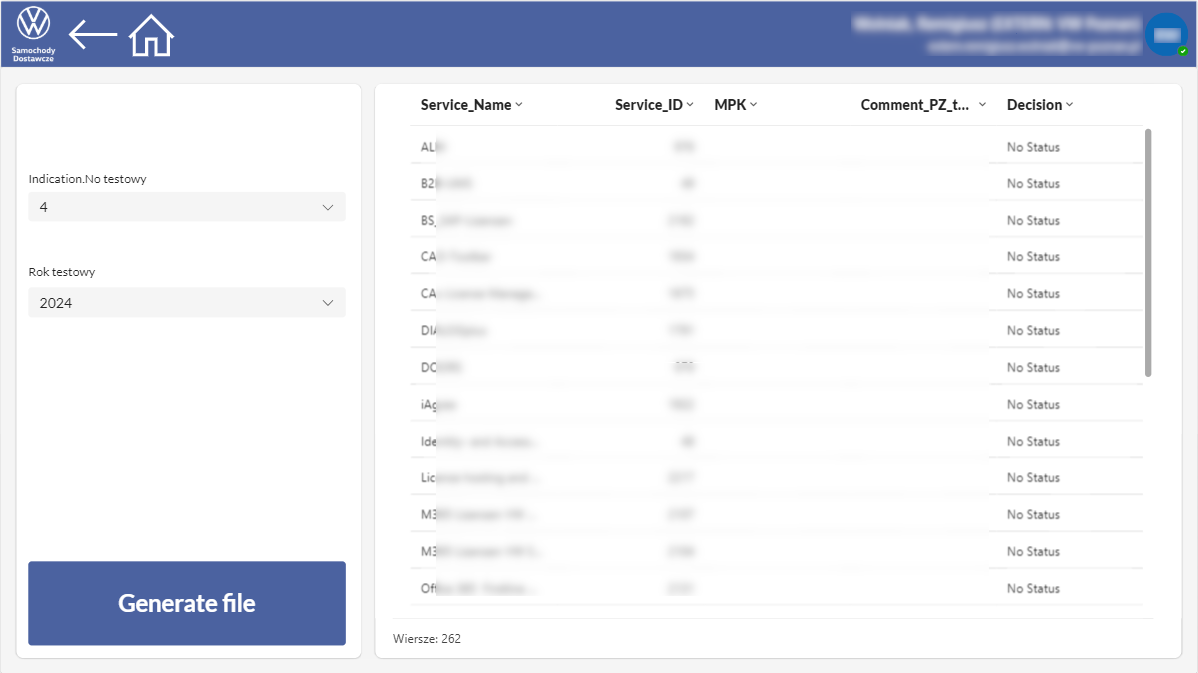
\includegraphics[width=0.9\textwidth]{figures/GenerateRaportForm.png}
%     \caption{Ekran generowania raportu}
%     \label{fig:generateraportform}
% \end{figure}

% Zebrane dane przechowywane są w tymczasowej kolekcji \emph{CombinedData}, która składa się z informacji z trzech źródeł, odpowiednio dopasowanych do wybranego przez użytkownika roku oraz indykacji. Przykładowy fragment kodu odpowiedzialnego za tworzenie tej kolekcji przedstawiono w listingu~\ref{lst:combineddata}:

\begin{lstlisting}[language=PowerFx, caption={Fragment kodu tworzącego kolekcję CombinedData}, label={lst:combineddata}] 
    ClearCollect(
    CombinedData;
    AddColumns(
        LocalServiceData;
        MPK;
        LookUp(
            LocalCostData;
            Service_ID = LocalServiceData[@Service_ID] && Year = Year_Dropdown_1.Selected.Value;
            MPK
        );
        Comment_PZ_to_WOB;
        LookUp(
            LocalIndicationsData;
            Service_ID = LocalServiceData[@Service_ID] && Year = Year_Dropdown_1.Selected.Value && IndicationNo = IndicationNo_Dropdown_1.Selected.Value;
            Comment_PZ_to_WOB);     
    [...]
);;

\end{lstlisting}

Kod ten korzysta z następujących funkcji:
\begin{itemize}
    \item \emph{ClearCollect} -- przypisuje dane do kolekcji o podanej nazwie,
    \item \emph{AddColumns} -- pozwala na dodanie do kolekcji nowej kolumny i formuły definiującej jej wartości,
    \item \emph{LookUp} -- wyszukuje rekordy w tabeli na podstawie podanych kryteriów.
\end{itemize}

\subsection{Przekazywanie danych do Power Automate}

W lewym dolnym rogu interfejsu znajduje się przycisk \emph{Generate file}, który po naciśnięciu uruchamia przepływ Power Automate, odpowiedzialny za stworzenie pliku na podstawie danych wejściowych. Dane te są przekazywane do usługi Power Automate w postaci ciągu tekstowego, sformatowanego jako JSON\footnote{JSON - format wymiany danych, który jest oparty na strukturze tekstowej}, wykorzystując połączone informacje z trzech źródeł zawarte w kolekcji \emph{CombinedData}. Kod wywołujący funkcję \emph{GenerateRaport} przedstawiono w listingu~\ref{lst:generateraport}.



\begin{lstlisting}[language=PowerFx, caption={Kod wywołujący funkcję GenerateRaport}, label={lst:generateraport}]
    GenerateRaport.Run(
        Substitute(
            "[" & 
            Concat(
                CombinedData;
                "{""Service_ID"":""" & Service_ID & """," &
                """Service_Name"":""" & Service_Name & """," &
                """MPK"":""" & MPK & """," &
                """Comment_PZ_to_WOB"":""" & Comment_PZ_to_WOB & """," &
                """Decision"":""" & Decision & """},"
            ) & 
            "]",
            "},]"; 
            "}]"
        ),
        IndicationNoCollect.Value,
        YearNoCollect.Value
    )
    \end{lstlisting}



\subsection{Generowanie raportu w Power Automate}


\emph{Flow} o nazwie \emph{GenerateRaport} składa się z kilku komponentów, które 
pozwalają na stworzenie raportu w formacie arkusza kalkulacyjnego, w oparciu o dane z list SharePoint. Przepływ ten zawiera następujące instrukcje:

\begin{itemize}
    \item \textbf{Wejście danych:} \emph{Flow} przyjmuje trzy dane wejściowe: ciąg znaków w formacie JSON, zawierający dane przekazane z aplikacji do przetworzenia, wybraną indykację oraz wybrany rok.
    \item \textbf{Inicjalizacja zmiennej:} W tym kroku tworzona jest zmienna odpowiedzialna za nazwę generowanego pliku. Zmienna zawiera dynamicznie generowaną datę utworzenia pliku.
    \item \textbf{Generowanie pustego arkusza Excel:} Wykorzystywany jest statyczny plik Excel, zapisany w formacie Base64, który pełni rolę szablonu dla dalszego przetwarzania.
    \item \textbf{Tworzenie pliku na SharePoint:} Szablon arkusza zostaje zapisany w określonej lokalizacji w bibliotece SharePoint.
    \item \textbf{Sprawdzenie dostępności pliku:} W celu upewnienia się, że plik jest gotowy do dalszego przetwarzania, uruchamiana jest pętla \emph{Do until}, która weryfikuje dostępność pliku na platformie.
    \item \textbf{Uruchomienie skryptu:} Na końcu przepływu wywoływany jest skrypt pakietu office, który generuje wypełniony arkusz Excel.
\end{itemize}

Schemat \ref{fig:generateflowcomponent} przedstawia szczegółowy schemat przepływu, uwzględniający poszczególne kroki oraz przepływ danych między nimi.

\begin{figure}[H]
    \centering
    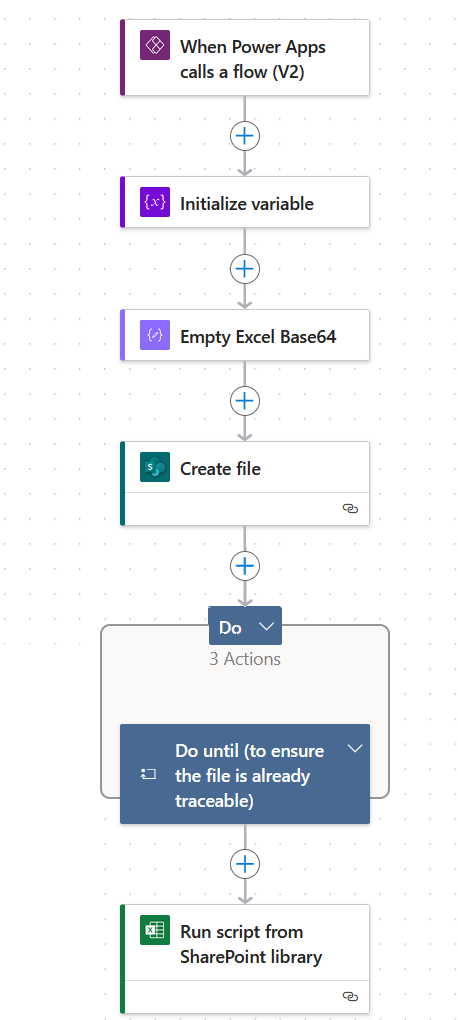
\includegraphics[width=0.45\textwidth]{figures/GenerateRaportFlow.png}
    \caption{Schemat przepływu \emph{GenerateRaport}}
    \label{fig:generateflowcomponent}
\end{figure}

\subsubsection*{Opis działania skryptu generującego raport}

Skrypt odpowiedzialny za generowanie raportu wykonuje kilka operacji. Jego główne funkcje to:
\begin{itemize}
    \item \textbf{Analiza danych wejściowych:} Przyjęcie danych w formacie JSON oraz roku. W przypadku otrzymania niepoprawnych dancyh, w arkuszu umieszczony jest odpowiedni komunikat.
    \item \textbf{Tworzenie arkusza:} Sprawdzenie, czy arkusz wynikowy już istnieje -- jeśli tak, to usuwa go i tworzy nowy.
    \item \textbf{Dynamiczne wstawianie danych:} Kolumny zawierające informacje na temat cen, mają w nagłówkach podany rok, których one dotyczą.
    \item \textbf{Generowanie tabeli:} Tworzenie nagłówków tabel (np. \texttt{Service\_ID}, \texttt{Service\_Name}) oraz wprowadzenie danych wypełniające tabelę, pobierane z JSON.
    \item \textbf{Formatowanie:} Skrypt aktywuje opcję filtracji kolumn oraz zmienia ich szerokość. Dzięki temu arkusz jest czytelny i nie wymaga formatowania ze strony użytkownika.
\end{itemize}




